A tester consists of a validator and a test harness.  Chapters~\ref{chap:theory}
and \ref{chap:practices} have explained the validator's theory and practices.
In this chapter, I present a language-based design for test harnesses, showing
how to generate and shrink test inputs effectively and address inter-execution
nondeterminism.

\autoref{sec:harness-overview} provides a brief overview of how test harnesses
work.  \autoref{sec:heuristics} explains how to write heuristics to generate
interesting test inputs.  \autoref{sec:shrinking} then shows a shrinking
mechanism that keeps the test inputs interesting among different executions.

\section{Overview}
\label{sec:harness-overview}
\begin{figure}
  \centering
  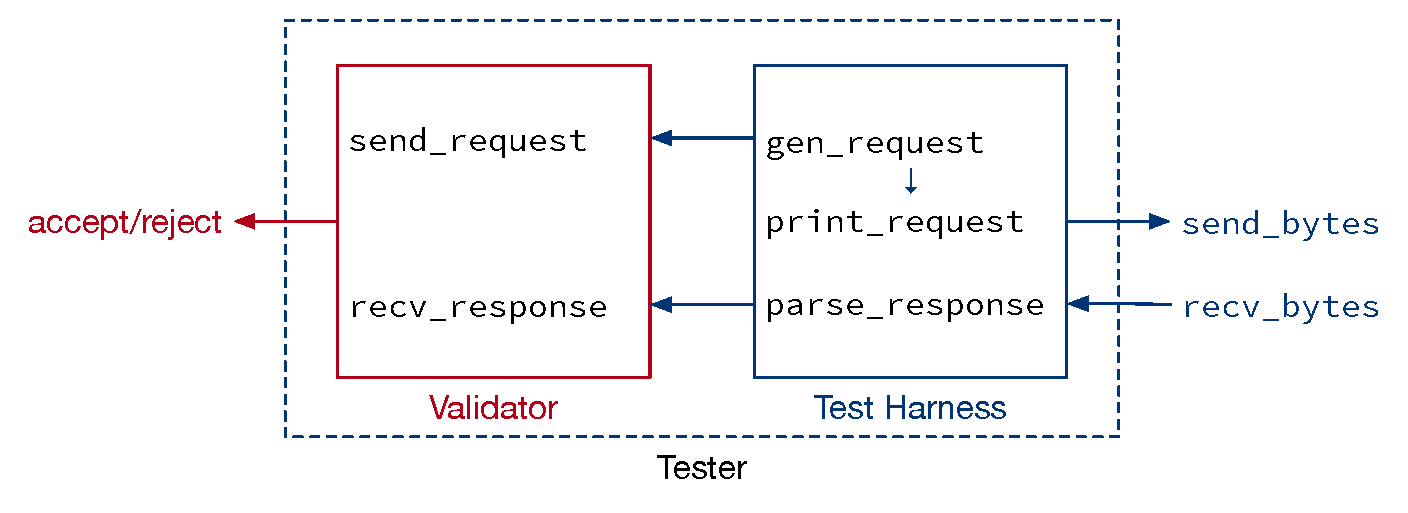
\includegraphics[width=.9\textwidth]{figures/harness-outline}
  \caption{Tester architecture outline.}
  \label{fig:overview}
\end{figure}

This section introduces the abstract architecture of an interactive tester,
using the networked server as an example.  I'll present a na\"ive implementation
of the test harness, which will be improved in the following sections.

The test harness interacts with the environment and provides the observations
for the validator.  The validator may represent requests and responses as
abstract datatypes for the convenience of specification.  The test harness
translates these abstract representations into bytes transmitted on the
underlying channel.

As shown in \autoref{fig:overview}, when the validator wants to observe a sent
request, the harness generates the request and encodes it into bytes to send.
Conversely, when the validator wants to observe a received response, the harness
receives bytes from the environment and decodes them into abstract messages.

\begin{figure}
\begin{lstlisting}[numbers=left]
Definition gen_packet: IO concrete_packet :=
  src          <- random_conn;;
  method       <- oneof [Get; Put];;
  target       <- random_path;;%\label{line:random-path}%
  precondition <- oneof [IfMatch, IfNoneMatch];;
  etag         <- random_etag;;
  payload      <- random_string;;
  ret { Source      := src;
        Destination := server_conn;
        Data        := inr { Method     := method;
                             TargetPath := target;
                             Headers    := [(precondition, etag)];
                             Payload    := payload
                           }
      }.
\end{lstlisting}
\caption{Na\"ive generator for HTTP requests.}
\label{fig:naive-generator}
\end{figure}

A generator is a randomized program that produces test inputs.  One example is
the \ilc{gen_packet} function in \autoref{fig:execute}.  The HTTP packet
generator can be na\"ively implementation as shown in
\autoref{fig:naive-generator}.  It fills in the request's fields with arbitrary
values, and has limited coverage of the SUT's behavior.  This is because the
request target and ETags are both generated randomly, but a request is
interesting only if its ETag matches its target's corresponding resource stored
on the server.  A randomly generated request would result in 404 Not Found and
412 Precondition Failed in almost all cases.

To reveal more interesting behavior from the SUT, we should tune the generator's
distribution to emphasize certain patterns of the test input.  For example, if
the tester knows the set of paths where the server has stored resources, then it
can generate more paths that correspond to existing resources; if the tester has
observed some ETags generated by the server, then it can include these ETags in
future requests.  In the next section, I'll explain how to implement such
heuristics in ITree-based testers.


\section{Heuristics for Test Generation}
\label{sec:heuristics}
This section implements heuristics for generating test inputs.  I'll use the
HTTP tester as an example to show how to make requests more interesting by
parameterizing them over the model state (\autoref{sec:heuristic-state}) and the
trace (\autoref{sec:heuristic-trace}).

\subsection{State-based heuristics}
\label{sec:heuristic-state}
\paragraph{Motivation}
The model state may instruct the test generator to produce more interesting test
inputs.  For example, consider the \ilc{random_path} generator in
\autoref{line:random-path} of \autoref{fig:naive-generator}.  One way to improve
it is to generate more paths that have corresponding resources on the server:
\begin{coq}
  Definition gen_path (state: list (path * resource)) : IO path :=
    let paths: list path := map fst state in
    freq [(90, oneof paths);
          (10, random_path)].
\end{coq}

Here I modify the server model's state type \ilc{sigma} from \ilc{(path ->
  resource)} in \autoref{fig:if-match-server} into \ilc{(list (path *
  resource))}, which allows the generator to access the list of all \ilc{paths}
  in the server state.  The generator chooses from these existing paths in 90\%
  of the cases, as assigned by the \ilc{freq} combinator.  The remaining 10\%
  are still generated randomly, to discover how the SUT handles nonexistent
  paths.

For the \ilc{gen_packet} generator in \autoref{fig:naive-generator}, replacing
its \ilc{random_path} with the improved \ilc{gen_path} would generate more
interesting request targets.  This requires the \ilc{gen_packet} function to
carry the server state to instantiate \ilc{gen_path}.

As shown in \autoref{fig:backtrack}, the \ilc{GenPacket} generator is triggered
when the tester wants to observe a packet from itself to the SUT.
\autoref{fig:symbolic-observer} then shows that such \ilc{FromObserver} expectation
happens when the symbolic model \ilc{Send}s a packet.  Such a \ilc{Send} event
only happens when the server wants to receive a packet in
\autoref{fig:net-compose}.  The \ilc{Recv} events are triggered by the server
model in \autoref{fig:if-match-server}, which iterates over the server state
\ilc{sigma}.

\paragraph{Implementation}
To expose the server state to the request generator, I extend the symbolic
server model's \ilc{Recv} event type on Page~\pageref{def:symbolic-qae} to
include the server state:
\begin{coq}
  Variant qaE: Type -> Type :=
    Recv : sigma      -> qaE packet
  | Send : packet -> qaE unit.
\end{coq}

Now when the server wants to receive a request, it triggers \ilc{(Recv state)},
where \ilc{(state: sigma)} contains the server's paths and resources at that
point.  The \ilc{state} argument is then carried to the generator, by adding
parameters to the event types along the interpretation:
\begin{coq}
  Variant netE: Type -> Type :=
    Emit  : packet -> netE unit
  | Absorb: sigma      -> netE packet.

  Variant observeE : Type -> Type :=
    FromObserver   : sigma -> observeE concrete_packet
  | ToObserver     : observeE concrete_packet.

  Variant genE: Type -> Type :=
    GenPacket : sigma -> genE concrete_packet
  | GenBool   : genE bool.

  Definition gen_packet: sigma -> IO concrete_packet.
\end{coq}

\begin{figure}
\includegraphics[width=.6\linewidth]{figures/stategen}
\caption{State-based heuristics.}
\label{fig:stategen}
\end{figure}

As a result, when instantiating the \ilc{(GenPacket state)} event in
\autoref{fig:execute}, we can feed the \ilc{gen_packet} function with argument
\ilc{state}, so that \ilc{gen_path} can generate interesting paths based on the
server state.  \autoref{fig:stategen} illustrates this state-based heuristics.
It refines the test harness box in \autoref{fig:overview}, and will be extended
with trace-based heuristics in the next subsection.

\subsection{Trace-based heuristics}
\label{sec:heuristic-trace}

When the SUT makes internal choices, \eg, generating ETags, the
specification represents them as symbolic variables.  These variables' concrete
value are not stored in the specification state, but may be observed during
execution.  For example, when an HTTP server responds to a GET request, it might
include the resource's ETag as shown in \autoref{sec:internal-nondeterminism}.

To improve the generator in \autoref{fig:naive-generator}, we can generate
interesting ETags based on the trace produced during execution.  The trace is a
list of packets sent and received by the tester, and the packets' payloads may
include responses that have an ETag field.  The \ilc{gen_etag} function
emphasizes ETags that were observed in the trace, which are more likely to match
those generated by the SUT:
\begin{coq}
  Definition gen_etag (trace: list concrete_packet) : IO string :=
    let etags: list string := tags_of trace in
    freq [(90, oneof etags);
          (10, random_etag)].
\end{coq}

To utilize this improved generator for ETags, the tester needs to record the
trace of packets sent and received.  This is done by modifying the \ilc{execute}
function in \autoref{fig:execute}, adding an accumulator called ``\ilc{trace}''
as the recursion parameter:
\begin{coq}
  Fixpoint execute (fuel: nat) (trace: list concrete_packet)
                   (m: itree tE void) : IO bool :=
    match fuel with
    | S fuel' =>
      match m with
      | Impure e k =>
        match e with
        | (ClientSend q|) => client_send q;;
                             execute fuel' (trace ++ [q]) (k tt)
        | (ClientRecv|)   => oa <- client_recv;;                             
                             let trace' := match oa with
                                           | Some a => trace ++ [a]
                                           | None   => trace
                                           end in
                             execute fuel' trace' (k oa)
        | (|GenPacket state|) => pkt <- gen_packet state trace;;
                                 execute fuel' trace (k pkt)
        ... (* similar to %\autoref{fig:execute}% *)
\end{coq}
\lys{\ilc{trace ++ [q]} is indeed less inefficient than storing a reversed trace,
but this code is to show the concept of ``appending'' requests and responses to
a trace, and assumes that readers have the ability of optimizing its
performance.}

When the tester sends or receives a packet, the packet is appended to the
runtime \ilc{trace}.  Then the \ilc{gen_packet} generator can take the trace
accumulated so far and feed it to the ETag generator:
\begin{coq}
  Definition gen_packet (state: sigma) (trace: list concrete_packet) :=
    target <- gen_path state;;
    etag   <- gen_etag trace;;
    ... (* same as %\autoref{fig:naive-generator}% *)
\end{coq}

\begin{figure}
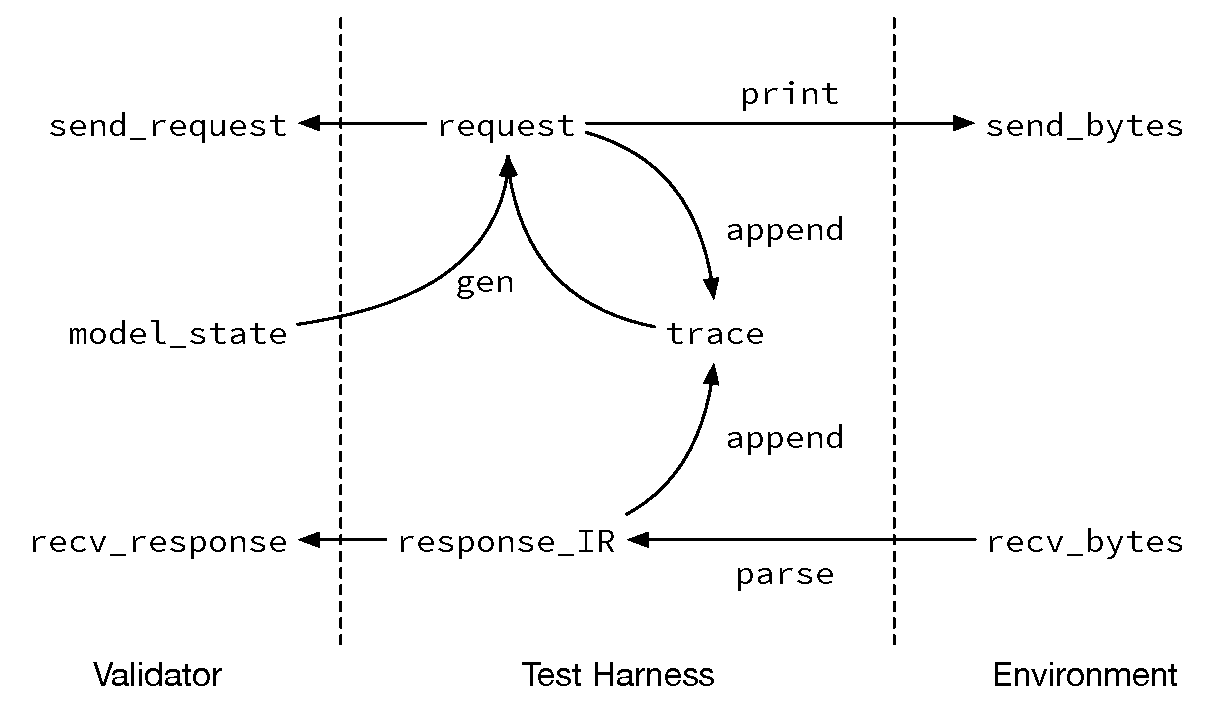
\includegraphics[width=.7\linewidth]{figures/gen}
\caption{Combining state-based and trace-based heuristics.}
\label{fig:gen}
\end{figure}

Now we can generate interesting test inputs by combining state-based and
trace-based heuristics, as shown in \autoref{fig:gen}.  In the next section,
I'll further extend this framework and shrink the test inputs while keeping them
interesting, addressing inter-execution nondeterminism.


\section{Shrinking Interactive Tests}
\label{sec:shrinking}
Suppose we have generated a test input that has caused invalid observations of
the SUT.  The generated counterexample consists of (1) {\em signal} that is
essential to triggering violations, and (2) {\em noise} that does not contribute
to revealing such violations.  We need to shrink the counterexample by removing
the noise and keeping the signal.

For interactive testing, the test input is a sequence of request messages.  An
intuitive way of shrinking is to remove some requests from the original sequence
and rerun the test.  However, rerunning an interesting request might produce
trivial results, due to inter-execution nondeterminism discussed in
\autoref{sec:inter-execution}.

To prevent turning signal into noise when rerunning the test, I shrink the
heurestics instead of shrinking the generated test input.
\autoref{sec:shrink-architecture} introduces the architecture for interactive
shrinking, then \autoref{sec:shrink-ir} explains the language design beneath
that addresses inter-execution nondeterminism.

\subsection{Architecture}
\label{sec:shrink-architecture}

I propose a generic framework for generating and shrinking interactive tests.
The key idea is to introduce an abstract representation for test inputs that
embeds trace-based heuristics.  When shrinking the counterexample, the test
harness picks a substructure of the abstract representation, and computes the
corresponding test input using the new runtime trace.

For example, when generating a timestamp, instead of producing concrete value,
e.g., ``\httpdate\today~\currenttime~GMT'', the generator returns an abstract
representation that says ``use the timestamp observed in the last response''.
When rerunning the test, the timestamp is computed from the new trace, e.g.,
``\httpdate\DayAfter~\currenttime~GMT''.

\begin{figure}
  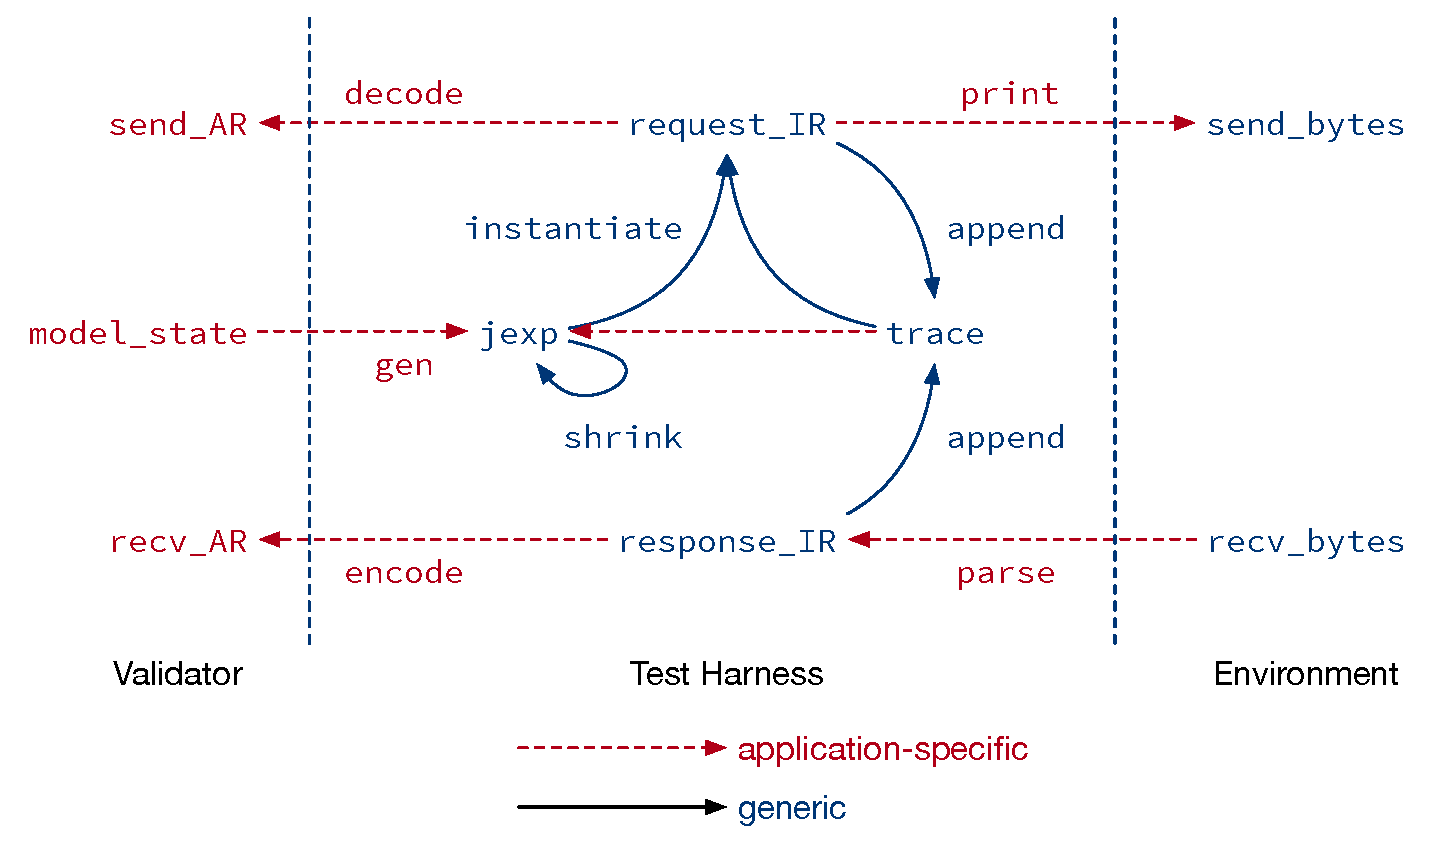
\includegraphics[width=.8\textwidth]{figures/shrink}
  \caption{Complete architecture of the test harness.}
  \label{fig:shrink}
\end{figure}

The test generation and shrinking framework is shown in \autoref{fig:shrink}.
It involves four languages, from right to left:
\begin{enumerate}
  \item Byte representation, in which the tester interacts with the environment.
    This can be network packets, file contents, or other serialized data
    produced and observed by the tester.
  \item Intermediate representation (IR), a generic language that abstracts the
    byte representation as structured data.  The test harness {\em parses} byte
    observations and records its trace in terms of the IR, which allows
    representing trace-based heuristics as a generic language, i.e.,
    J-expressions.
  \item J-expression (Jexp), a symbolic abstraction of the IR.  The IR
    corresponds to concrete inputs and outputs, whereas Jexp defines a
    computation from trace to IR.  The generator provides test inputs in terms
    of Jexps; The test harness {\em instantiates} the generated Jexps into
    request IR, and {\em prints} them into byte representation.

    When shrinking test inputs, the test harness shrinks the sequence of Jexps.
    The shrunk Jexps are then instantiated by the new trace during runtime.

    The intermediate representation and J-expression will be further explained
    in \autoref{sec:shrink-ir}.
  \item Application representation (AR), including the request (\ilc Q),
    response (\ilc A), and state (\ilc S) types used for specifying the
    protocol.  Specification writers can choose the type interface at their
    convenience, provided the request and response types are embeddable into the
    IR.
\end{enumerate}

The testing framework implements protocol-independent mechanisms like recording
the trace and shrinking counterexamples, which correspond to the blue solid
arrows in \autoref{fig:shrink}.  It can be used for testing various protocols,
provided application-specific translations from IR to AR and between IR and
bytes, illustrated as red dotted arrows.  The test developer needs to tune the
generator that produces Jexps, encoding their domain knowledge as state-based
and trace-based heuristics.

\subsection{Abstract representation languages}
\label{sec:shrink-ir}
I choose JSON as the IR in this framework, which allows syntax trees to be
arbitrarily wide and deep, and provides sufficient expressiveness for encoding
message data types in general.

\begin{figure}
\[\begin{array}{r@{\;}l}
\mathsf{JSON^T}\triangleq&\mathsf T\mid\{\mathsf{object^T}\}\mid[\mathsf{array^T}]\mid\mathsf{string}\mid\Int\mid\Bool\mid\mathsf{null}\\
\mathsf{object^T}\triangleq&\nil\mid\mathsf{"string": JSON^T,object^T}\\
\mathsf{array^T}\triangleq&\nil\mid\mathsf{JSON^T,array^T}\\
\mathsf{IR}\triangleq&\mathsf{JSON^{IR}}\\
\mathsf{Jexp}\triangleq&\mathsf{JSON^{\Jref{\Label}{\Jpath}{\Function}}}\\
&\text{where }\Label\in\Nat,\Function\in\mathsf{IR}\to\mathsf{IR}\\
\Jpath\triangleq&\This\mid\Jpath\Number\Index\mid\Jpath\At\Field\\
&\text{where }\Index\in\Nat,\Field\in\mathsf{string}
\end{array}\]
\caption{Intermediate representation and J-expression.}
\label{fig:ir-jexp}
\end{figure}

\begin{figure}
\begin{minipage}{.6\textwidth}
\begin{coq}
Notation   labelT := nat.
Definition traceT := list (labelT * IR).

Context q1 q2 a1 a2 : IR.
Example labelled_trace: traceT :=
  [(1, q1); (3, q2); (4, a2); (2, a1)].
\end{coq}
\end{minipage}\begin{minipage}{.3\textwidth}
  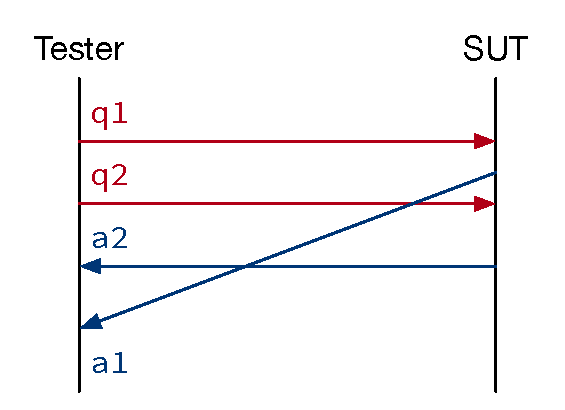
\includegraphics[width=\linewidth]{figures/ir-trace}
\end{minipage}
\caption{Labelled trace example.}
\label{fig:ir-trace}
\end{figure}

\begin{figure}
  \begin{minipage}[t]{.4\textwidth}
\begin{json}
  (* a2 = *)
  {
    "files": [
      {
        "name": "foo",
        "mode": 755
      },
      {
        "name": "bar",
        "mode": 500
      }
    ],
    "exitCode": 0
  }
\end{json}
  \end{minipage}\begin{minipage}[t]{.5\textwidth}
\begin{coq}
(* Jpath syntax defined in %\autoref{fig:ir-jexp}%. *)
Example second_file_mode: jpath :=
  this @ "files" # 2 @ "mode".

Example mode_add_write (j: IR) : IR :=
  match j with
  | JSON_Number n =>
    JSON_Number (mode_bits_or 200 n)
  | _ => j
  end.

Example id (j: IR) : IR := j.
\end{coq}
  \end{minipage}
  \caption{IR, Jpath, and heuristics function example.}
  \label{fig:ir-jpath}
\end{figure}

\paragraph{Syntax}
The J-expression is an extension of JSON that can encode trace-based heuristics.
As shown in \autoref{fig:ir-jexp}, a Jexp may include syntax
$(\Label.\Jpath.\Function)$ that represents trace-based heuristics, specified as:
\begin{enumerate}
\item The test harness records the trace as a list of labelled messages, where
  the requests are labelled odd, and their responses are labelled as the next
  even number.  The $\Label$ in a Jexp locates the IR in the trace with which
  the heuristics computes the input.  Labelling messages allows the reproducing
  trace-based heuristics despite shrinking and inter-execution nondeterminism.

  For example, consider the trace in \autoref{fig:ir-trace}: If a trace-based
  heuristics is interested in \ilc{q2}'s response \ilc{a2}, then it can be
  encoded as ``compute the test input based on message labelled 4'':
\begin{coq}
  Context get_label: labelT -> traceT -> IR.

  Compute get_label 4 labelled_trace.
  (* = a2 : IR *)
\end{coq}
  
  Suppose the test input is shrunk by removing \ilc{q1}, the label for \ilc{q2}
  remains unchanged as 3, so label 4 corresponds to the new response to
  \ilc{q2}:
\begin{coq}
  Example new_trace: traceT :=
    [(3, q2); (4, a2')].

  Compute get_label 4 new_trace.
  (* = a2' : IR *)
\end{coq}

As a result, the trace-based heuristics are preserved and adapted to new
executions during the shrinking process.
\item The $\Jpath$ is a path in the IR's syntax tree, and refers to a
  substructure of the IR that the heuristics uses.

  For example, suppose request \ilc{q2} lists files in a directory using the
  POSIX \inlinec{ls} command, and its response \ilc{a2} is encoded as the IR
  shown in \autoref{fig:ir-jpath}.  The response IR is a JSON object whose
  \inlinec{"files"} field is an array of objects, each has a \inlinec{"name"}
  and a \inlinec{"mode"} field.  A heuristic can refer to the second file's
  mode bits by Jpath \ilj{(this@"files"#2@"mode")}, which will guide the test
  harness to locate its corresponding value:
\begin{coq}
  Context get_jpath: jpath -> IR -> IR.

  Compute get_jpath second_file_mode a2.
  (* = JSON_Number 500 : IR *)
\end{coq}
\item The $\Function$ has type $(\mathsf{IR}\to\mathsf{IR})$, and defines the
  computation based on the sub-IR located by the Jpath.

  Consider the mode bits located in the previous example: If the heuristic
  wants to add write permission to the mode bits, it can do so with the
  \ilc{mode_add_write} function in \autoref{fig:ir-jpath}, which produces mode
  700.  Some heuristics might use the sub-IR 500 as-is, using the identity
  function \ilc{id}.
\end{enumerate}

\paragraph{Semantics}
J-expression provides a generic interface for test developers to implement
trace-based heuristics.  For the aforementioned file system example, the tester
can generate a request that changes the mode bits of an observed file, with the
following Jexp:
\begin{json}
  (* e5 = *)
  {
    "command": "chmod",
    "args": [
      4.(this@"files"#2@"mode").mode_add_write,
      4.(this@"files"#2@"name").id
    ]
  }
\end{json}

To instantiate Jexps into request IR, the test harness substitutes all
occurences of $(\Jref{l}{p}{f})$ in the Jexp with its corresponding IR computed
from the runtime trace:
\begin{coq}
  Definition eval (l: labelT) (p: jpath) (f: IR -> IR) (t: traceT) : IR :=
    let a: IR := get_label l t in
    let j: IR := get_jpath p a in
    f j.
\end{coq}

For example, given the runtime trace in \autoref{fig:ir-trace}, with \ilc{a2} is
defined in \autoref{fig:ir-jexp}, the the above Jexp is instantiated into the
following request:

\begin{json}
  (* instantiate e5 labelled_trace = *)
  { 
    "command": "chmod",
    "args": [ 700, "bar" ]
  }
\end{json}

However, when rerunning the test, the \ilc{new_trace} has a different response
associated with label 4.  The new response \ilc{a2'} might have fewer than 2
files in its payload.  Moreover, the response \ilc{a2'} might have not appeared
in the trace, due to delays in the environment.

To instantiate the original Jexp in such situations, I loosen the
\ilc{get_jpath} and \ilc{get_label} functions when evaluating the heuristics:
\begin{enumerate}
\item When evaluating a Jpath starting with \ilj{p#n}, if \ilj p corresponds to
  an array with fewer than \ilj n elements, or the array's \ilj n-th element
  cannot properly evaluate the remaining path, then try continuing the
  evaluation with any other element in the array.

  For example, consider evaluating \ilj{(this@3#"bar")} on the following IR's:
  \begin{center}
\begin{minipage}[t]{.5\linewidth}
\begin{json}
  (* j2 = *)
  [
    { "foo": 21 },
    { "bar": 22 }
  ]
\end{json}
\end{minipage}\begin{minipage}[t]{.5\linewidth}
\begin{json}
  (* j3 = *)
  [
    { "bar": 31 },
    { "baz": 32 },
    { "foo": 33 }
  ]
\end{json}
\end{minipage}
  \end{center}

  Here \ilj{j2} doesn't have a third element, and \ilj{j3}'s third element
  doesn't have field \ilj{"bar"}.  In these cases, \ilj{get_jpath} chooses other
  elements in the two arrays, resulting in value \ilj{22} for \ilj{j2}, and
  \ilj{31} for \ilj{j3}.
  
\item When evaluating label \ilj l and Jpath \ilj p on a trace, if the message
  labelled \ilj l does not exist in the trace, or cannot evaluate Jpath \ilj p
  properly, then try continuing the evaluation with any other IR in the trace.

  For example, consider evaluating J-expression \ilj{6.(this#2@"foo").id} on the
  following traces:
\begin{coq}
  Definition t1: traceT :=
    [(1,q1); (2,j2); (5,q2)].

  Definition t2: traceT :=
    [(3,q1); (4,j3); (5,q2); (6,a2)].
\end{coq}

Here \ilj{t1} doesn't have a message labelled 6, probably caused by environment
delays; \ilj{t2} has label 6 but its corresponding message is an object rather
than an array expected by the Jexp.  In these cases, \ilc{eval} chooses other
messages in the trace to evaluate, resulting in value \ilc{21} for \ilc{t1}, and
\ilc{33} for \ilc{t2}.
\end{enumerate}

By introducing loose evaluation of J-expressions, my test harness allows partial
instantiation of heuristics when the runtime trace is less than satisfying.

So far I have shown how to generate and shrink interactive test inputs and
address inter-execution nondeterminism.  In the next chapter, I'll combine this
test harness design with the validator practice in \autoref{chap:practices}, and
evaluate these techniques by testing real-world systems like HTTP servers and
file synchronizers.

